\documentclass[]{article}

\usepackage{tikz}
\usepackage{amsmath}
\usepackage{amsfonts}
\usepackage{amssymb}
\usepackage{tkz-euclide}
\usepackage{xcolor}
\usepackage{pgfplots}

% Required package
\usetikzlibrary{positioning}
\usetikzlibrary{svg.path}
\usetikzlibrary{arrows}
\usetikzlibrary{shapes.geometric,calc}

\newdimen\XCoord
\newdimen\YCoord
\newcommand*{\ExtractCoordinate}[1]{\path (#1); \pgfgetlastxy{\XCoord}{\YCoord};}%

%opening
\title{Computed Torque Control}
\author{Glen Henshaw\\Craig Carignan}

\begin{document}

\maketitle


\section{Intro}
Here's a block diagram of our robotic system:
\begin{figure}[h!]
 \centering
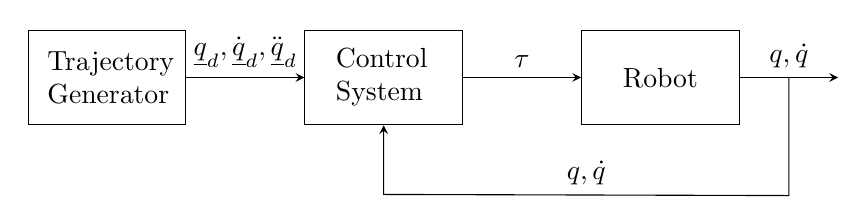
\begin{tikzpicture}
 % Sum shape
 \node[draw, 
        minimum width=2cm,
        minimum height=1.2cm
        ] (trajgen) at (0,0){\parbox[t]{0.125\linewidth}{Trajectory\\Generator}};

% Controller
\node [draw,
    minimum width=2cm,
    minimum height=1.2cm,
    right=1.5cm of trajgen
]  (controller) {\parbox[t]{0.1\linewidth}{Control\\System}};
 
% System H(s)
\node [draw,
    minimum width=2cm, 
    minimum height=1.2cm,
    right=1.5cm of controller
] (system) {Robot};
  
% Arrows with text label
%\draw[-stealth] (trajgen.north east) -- (controller.north west)
%    node[midway,above]{$\Omega$};
\draw[-stealth] (trajgen.east) -- (controller.west)
    node[midway,above]{$\underline{q}_{d}, \dot{\underline{q}}_{d}, \ddot{\underline{q}}_{d}$};
%\draw[-stealth] (trajgen.south east) -- (controller.south west)
%    node[midway,above]{$\ddot{\Omega}$};
 
\draw[-stealth] (controller.east) -- (system.west) 
    node[midway,above]{$\tau$};

\draw[-stealth] (system.east) -- ++ (1.25,0) 
    node[midway](output){}node[midway,above]{$q, \dot{q}$};

\ExtractCoordinate{controller.south}
\draw[-stealth] (output.center) -- ++ (0,-1.5) -- (\XCoord, \YCoord-25) node[midway,above]{$q, \dot{q}$} -- (controller.south);

%\draw[-stealth] (output.center) -- ++ (0,-2) -- (\XCoord-10, \YCoord-37) node[midway,above]{$\dot{q}$} -- (controller.south west);

  
\end{tikzpicture}
\end{figure}

And remember from last time that we can write the dynamics of our robot in the form
\begin{equation}
 \underline{\tau} = M(\underline{q}) \ddot{\underline{q}} +C(\underline{q}, \underline{\dot{q}})\dot{q} + E(\underline{q}, \underline{\dot{q}}) \label{hamiltonian}
\end{equation}

\section{Gain scheduling}
Remember last time we decided to pretend that our dynamics were uncoupled and linear:
\begin{equation}
 \tau_{i} = m_{i}\ddot{q}_{i} + c_{i}\dot{q}_{i}+e_{i}(q_{i}) \label{SMD}
\end{equation}
and we talked about some limitations of that approach. It really only works when either the mass matrix is mostly diagonal and when the joint velocities are relatively low. But it has another problem that we didn't talk about, which is that the full dynamics given in Equation \ref{hamiltonian} vary with arm pose, whereas the simplified dynamics given in Equation \ref{SMD} don't. As a consequence, EVEN IF you assume that the dynamics really are uncoupled, the $m_{i}$, $c_{i}$, and $e(\cdot)$ terms in Equation \ref{SMD} change depending on where you are in the workspace. If you go through the exercise we did last lecture where we designed an independent PD control law with a desired stiffness and critical damping, the values of $m_{i}$ and $c_{i}$ show up in the calculations for $k_{v}$ and $k_{p}$. If you calculate $k_{v}$ and $k_{p}$ for some given values of $m_{i}$ and $c_{i}$, but then servo the arm to a pose significantly different from the one you started with, you will suddenly not have a system with the desired stiffness or damping. What can you do about that?

One thing you can do is called ``robust controller design'', which in intuitive terms is a set of design techniques that help you choose gains that work for your problem over the entire range of $m_{i}$ and $c_{i}$ values your robot will assume. For instance, you could calculate both the minimum and maximum values of $m_{i}$ and $c_{i}$, pick a minimum and maximum stiffness and that you always want critical damping or overdamping -- in other words, that your damping constant $\zeta$ must always be less than 1 -- and then find a single set of gains that works.

With serial link manipulators, the range of effective masses you may ancounter can change so dramatically, though, that this is often a futile exercise. You will often be able to find a set of gains that works for your worst case, but it will be so overdamped for your ``average'' case that the robot can't really do what you need it to.

One very common way to handle this difficulty is through \textit{gain scheduling}. The idea here is that you pick different operating poses and/or different masses you will encounter -- e.g different values of $m_{i}$ and $c_{i}$ -- and calculate different values of $k_{v}$ and $k_{p}$ for each pose. You then switch gains in real time as you get closer to or farther away from different poses and/or as you pick up or drop different payloads.

Formally, this is a table:
\begin{table}[h!]
  \begin{center}
    \label{tab:table1}
    \begin{tabular}{lccc} % <-- Alignments: 1st column left, 2nd middle and 3rd right, with vertical lines in between
      \textbf{$m_{i}$} & \textbf{$c_{i}$} & \textbf{$k_{p}$} & \textbf{$k_{p}$} \\ 
      \hline
      1 & 2 & 5 & 3\\
      5 & 3 & 7 & 4\\
      3 & 1 & 6 & 3.5\\
    \end{tabular}
  \end{center}
\end{table}

This works pretty well for systems where the degrees of freedom are low, or where you don't need extremely high performance. It relies on the fact -- a surprisingly difficult to formally prove fact -- that linear PD control is unreasonably effective when applied to a nonlinear Hamiltonian system like a serial joint manipulator.

The major way in which gain scheduling fails is that the number of gain sets you need scales exponentially with the degrees of freedom. So, whereas it may be straightforward if somewhat tedious to find a complete gain schedule (e.g. one that gives you similar performance across the entire dexterous workspace) for a 3 DOF arm, it may become completely intractible for a 7 DOF arm. For instance, if you decided you need, say, ten gain sets for your three DOF arm, you would need ~10,000 gain sets for a 6 DOF arm and ~100,000 for a 7 DOF arm in order to get roughly equivalent performance.

Nevertheless, especially for manufacturing cell automation where the number of poses you will actually see are small, gain scheduling can be quite effective.

% \section{Trajectory--tracking Controllers}
% So far we've assumed we want the manipualtor to go to a setpoint and stay there. But what if we want it to follow a trajectory?
% 
% In that case we can try a controller like:
% \begin{equation}
%  \tau = \underline{\ddot{q}} + K_{v}\dot{\tilde{\underline{q}}} + K_{p}\tilde{\underline{q}}
% \end{equation}
%  substituting this into Equation \ref{hamiltonian}

\section{Computed Torque Control}
An alternative is to artificially try to ``cancel'' the arm's natural dynamics and replace them with ones you like better.

Recall that last time we talked about ``open--loop'' control, where our dynamics were
\begin{displaymath}
 \underline{\tau} = M(\underline{q}) \ddot{\underline{q}} +C(\underline{q}, \underline{\dot{q}})\dot{q} + E(\underline{q}, \underline{\dot{q}})
\end{displaymath}
and our controller was 
\begin{displaymath}
 \underline{\tau} = M(\underline{q}) \ddot{\underline{q}}_{d} +C(\underline{q}, \underline{\dot{q}})\dot{q}_{d} + E(\underline{q}, \underline{\dot{q}})
\end{displaymath}
and we said that trying this was a bad idea, because we never really knew the exact values of the mass, Coriolis, and centripetal matrices, and also because there was always noise in our system. But let's play with this idea for a minute. What if we actually did know $M$, $C$, and $E$? In that case we could consider a \textbf{closed--loop} control law of the form
\begin{equation}
 \underline{\tau} = M(\underline{q})( \ddot{\underline{q}}_{d}- K_{p}(\underline{q} - \underline{q}_{d}) - K_{v}(\underline{\dot{q}} - \underline{\dot{q}}_{d})) +C(\underline{q}, \underline{\dot{q}})\dot{q} + E(\underline{q}, \underline{\dot{q}})  \label{computedtorque}
\end{equation}
If we plug Equation \ref{computedtorque} into Equation \ref{hamiltonian} we get:
\begin{displaymath}
 M(\underline{q}) \ddot{\underline{q}} +C(\underline{q}, \underline{\dot{q}})\dot{q} + E(\underline{q}, \underline{\dot{q}}) =  M(\underline{q})( \ddot{\underline{q}}_{d}- K_{p}(\underline{q} - \underline{q}_{d}) - K_{v}(\underline{\dot{q}} - \underline{\dot{q}}_{d})) +C(\underline{q}, \underline{\dot{q}})\dot{q} + E(\underline{q}, \underline{\dot{q}})
 \end{displaymath}
 or
 \begin{displaymath}
 M(\underline{q})(\ddot{\underline{q}} - \ddot{\underline{q}}_{d} + K_{p}(\underline{q} - \underline{q}_{d})+ K_{v}(\underline{\dot{q}} + \underline{\dot{q}}_{d})) + C(\underline{q}, \underline{\dot{q}})(\dot{\underline{q}} - \dot{\underline{q}})  = 0 
\end{displaymath}
and if we define
\begin{eqnarray}
 \underline{\tilde{q}} & = & \underline{q}_{d} - \underline{q} \nonumber\\
 \underline{\dot{\tilde{q}}} & = & \dot{\underline{q}}_{d} - \dot{\underline{q}} \nonumber \\
 \underline{\ddot{\tilde{q}}} & = & \ddot{\underline{q}}_{d} - \ddot{\underline{q}} 
\end{eqnarray}
then we get 
\begin{displaymath}
 \underline{\ddot{\tilde{q}}} + K_{v}\underline{\dot{\tilde{q}}} + K_{p}\underline{\tilde{q}} = 0 
 \end{displaymath}
 e.g. we would get perfect spring--mass--damper dynamics. And since this is a second--order linear equation, we know how it behaves -- as long as we pick $K_{p}$ and $K_{v}$ correctly, it asymptotically approaches the origin. Note, also, that because we have complete control over $K_{p}$ and $K_{v}$, we can (and almost always do) choose them to be diagonal. Therefore, the dynamics actually are decoupled, e.g. they look like
 \begin{displaymath}
  \ddot{\tilde{q}}_{i} + k_{v,i}\dot{\tilde{q}}_{i} + k_{p,i}\tilde{q}_{i} = 0.
 \end{displaymath}

 
 \textbf{It is very important to note} that this equation we have derived is in fact a differential equation that describes the dynamics of the SERVO ERROR. This is not the dynamics of the actual robot; this is the equation that describes how the tracking error of the robot evolves over time. This is a game we often play in nonlinear controls: we try to come up with a control law that gives us a differential equation describing the evolution of the tracking error.
 
 Furthermore, calculating the ``model'' portion of this controller, 
 \begin{displaymath}
  M(\underline{q})\ddot{\underline{q}}_{d}  +C(\underline{q}, \underline{\dot{q}})\dot{q}_{d} + E(\underline{q}, \underline{\dot{q}}) 
 \end{displaymath}
is straightforward -- it just uses the recursive Newton--Euler dynamics equations from Lectures 13 and 14. This control law is therefore often referred to as a ``computed torque'' control law, and it is the second most frequently used controller design in robotics, after independent joint control. it is particularly valuable in cases where the robot needs to move quickly and accurately, possibly while handling large masses.

There are some issues with computed torque control, though, the primary one being that we never exactly know the model parameters, and so we can't ever perfectly cancel out the system's natural dynamics. So in practice a computed torque control law actually calculates
\begin{displaymath}
 \underline{\tau} = \hat{M}(\underline{q}) \ddot{\underline{q}}_{d}- K_{p}(\underline{q} - \underline{q}_{d}) - K_{v}(\underline{\dot{q}} - \underline{\dot{q}}_{d})) + \hat{C}(\underline{q}, \underline{\dot{q}})\dot{q}_{d} + \hat{E}(\underline{q}, \underline{\dot{q}})  
\end{displaymath}
where $\hat{M}$ is our best guess at the true $M$ matrix, adn so on. If you plug this controller into Equation \ref{hamiltonian}, you end up with the following servo error dynamics:
\begin{displaymath}
 \ddot{\tilde{q}} + K_{v}\dot{\tilde{q}} + k_{p}\tilde{q} = \hat{M}^{-1}\left[(M-\hat{M})\ddot{q} + (C-\hat{C})\dot{q} + (E-\hat{E})\right]
\end{displaymath}
and it's not immediately obvious what the solutions to this equation look like. In point of fact, as long as the right--hand side is small enough -- which is to say, of our model isn't terribly inaccurate -- then you can sort of imagine this system as a perturbed spring--mass--damper system, and you can intuitively see that such a system won't stay at the origin, but it \textit{will} stay near the origin. How near depends on the spring constant and the size of the perturbation. Calculating a bound on this requires \textit{Lyapunov theory}.

\section{Lyapunov Theory}
Lyapunov was a 19th century Russian mathematician who pioneered ways of understanding the behavior of nonlinear systems without needing to actually solve them, e.g. without needing to write down closed--form solutions to their differential equations. This is good, because in general we \textit{can't} solve nonlinear differential equations.

The fundamental insight here is that if you can write down an equation for the energy of a system, and if you can prove that the system always dissipates energy, then at the end of the day the system has to be ``well behaved''. A mechanical system with no energy, for instance, is stationary.

Lyapunov generalized this insight slightly. Lyapunov theory posits that if you can write down \textbf{any} function of the state of the system which is always positive except at the origin, and if the time derivative of this equation is always negative except at the origin, then the state has to asymptotically converge to zero. Such a function is called a Lyapunov function. If you think of a Lyapunov function as the energy of the system, or a sort of pseudo--energy of the system, then you'll have the right intuition.

So let's consider the following simplified system plus controller:
\begin{equation}
 m\ddot{x} = -b\dot{x} - kx \label{smd2}
\end{equation}
our old friend the spring--mass--damper system.
The total energy of this system is
\begin{equation}
 v = \frac{1}{2}m\dot{x}^{2} + \frac{1}{2}kx^{2} \label{smdenergy}
\end{equation}
and the derivative of this is
\begin{displaymath}
 \dot{v} = m\dot{x}\ddot{x}+kx\dot{x}
\end{displaymath}
we can substitute for $m\ddot{x}$ from Equation \ref{smd2} to get
\begin{equation}
 \dot{v} = -b\dot{x}^{2} \label{smdenergyderiv}
\end{equation}
Note that by inspection, Equation \ref{smdenergy} is always positive except at $x=0$, and Equation \ref{smdenergyderiv} is always negative except at $\dot{x}=0$. This implies that the energy in the system must always leave the system until it reaches exactly zero, after which it must remain there. Therefore, without every writing down an explicit solution to Equation \ref{smd2} we have proven that it must continuously lose energy until it reaches the origin, which is an attractive stable point.

Congratulations, you have just done your first nonlinear stability proof.

OK, let's scale up a bit and see if we can use this approach for the manipulator described by Equation \ref{hamiltonian} and a simplified computed--torque controller where we assume we know exactly the Coriolis and centripetal forces and the environmental forces but not the mass matrix. We will also assume that we want the manipulator to settle at $\underline{q}=0$, its home position. And in order to make the math easier, we'll also assume that our mass estimate $\hat{M}$ is constant. This is basically a linear PD control law with an extra term that tries to cancel out environmental forces like gravity. This is an extremely common control design in industrial manipulators.

So our controller is:
\begin{equation}
 \tau_{c} = \hat{M}\left(-K_{p}\underline{q} - K_{v}\dot{\underline{q}}\right) + E \label{simplect}
\end{equation}
Substituting Equation \ref{simplect} into Equation \ref{hamiltonian}, we get
\begin{eqnarray}
 M\ddot{\underline{q}} + C\dot{\underline{q}} + E & = & \hat{M}\left(-K_{p}\underline{q} - K_{v}\dot{\underline{q}}\right) + E \nonumber \\
 M\underline{\ddot{q}} + \hat{M}K_{p}\underline{q} + \hat{M}K_{v}\dot{\underline{q}} + C\dot{\underline{q}} & = & 0 \nonumber \\
\end{eqnarray}
Because of our godlike intelligence, we're going to pull a candidate Lyapunov function out of the air:
\begin{displaymath}
 V = \frac{1}{2}\dot{\underline{q}}^{T}M\underline{\dot{q}} + \frac{1}{2}\underline{q}^{T}\hat{M}K_{p}\underline{q}
\end{displaymath}
which is positive definite.

Taking the derivative, we get
\begin{eqnarray}
 \dot{V} & = & \frac{1}{2}\dot{\underline{q}}^{T}\dot{M}\dot{\underline{q}} + \underline{\dot{q}}^{T}M\underline{\ddot{q}} + \underline{q}^{T}\hat{M}K_{p}\dot{\underline{q}} \nonumber \\
 & = & \frac{1}{2}\underline{\dot{q}}\dot{M}\underline{\dot{q}} + \dot{\underline{q}}^{T}\left( -\hat{M}K_{p}\underline{q} - \hat{M}K_{v}\dot{\underline{q}}-C\dot{\underline{q}}\right) + \underline{q}^{T}\hat{M}K_{p}\dot{\underline{q}} \nonumber \\& = & \dot{\underline{q}}^{T}\left(\frac{1}{2}\dot{M} - C - \hat{M}K_{v}\right)\dot{\underline{q}} \nonumber \\
 & = & \dot{\underline{q}}^{T}\left( \frac{1}{2}\dot{M} - C\right)\dot{\underline{q}} - \dot{\underline{q}}^{T}\hat{M}K_{v}\dot{\underline{q}} \label{lyap1}
\end{eqnarray}
and, huh, we've got a weird term involving the derivative of the mass matrix and the Coriolis/centripetal forces. 

It turns out we can prove that this term is equal to zero. The kinetic energy of the manipulator system can be written in vector form as
\begin{displaymath}
 \dot{\underline{q}}^{T}M\dot{\underline{q}}
\end{displaymath}
Recall that power is the time derivative of kinetic energy. The power for this system can be written in vector form as
\begin{displaymath}
 P = \dot{\underline{q}}^{T}\left(\tau-E\right)
\end{displaymath}
which is simply the joint velocities times the external torques on the system. In this case, the external torques are the torques exerted by the controller plus the gravitational and other environmental forces. Therefore:
\begin{eqnarray}
\frac{1}{2}\frac{d}{dt}\left(\dot{\underline{q}} M\dot{\underline{q}}\right) & = & \dot{\underline{q}}^{T}\left(\tau-E\right) \nonumber \\
\frac{1}{2}\dot{\underline{q}}^{T}\dot{M}\dot{\underline{q}} + \dot{\underline{q}}^{T}M\underline{\ddot{q}} & = & \dot{\underline{q}}^{T}\left(\tau-E\right) \nonumber \\
\frac{1}{2}\dot{\underline{q}}^{T}\dot{M}\dot{\underline{q}} + \dot{\underline{q}}\left[\tau - C\dot{\underline{q}} - E\right] & = & \dot{\underline{q}}^{T}\left(\tau-E\right) \nonumber \\
\frac{1}{2}\dot{\underline{q}}^{T}\dot{M}\dot{\underline{q}} + \dot{\underline{q}}\left[\tau - C\dot{\underline{q}} - E\right] & = & \dot{\underline{q}}^{T}\left(\tau-E\right) \nonumber \\
\dot{\underline{q}}^{T}\left(\frac{1}{2}\dot{M} - C\right)\dot{\underline{q}} & = & 0 \nonumber
\end{eqnarray}
and this is the result we need. We can now cancel the term in Equation \ref{lyap1}
to get
\begin{eqnarray}
\dot{V} & = & \dot{\underline{q}}^{T}\left( \frac{1}{2}\dot{M} - C\right)\dot{\underline{q}} - \dot{\underline{q}}^{T}\hat{M}K_{v}\dot{\underline{q}} \nonumber \\
& = & - \dot{\underline{q}}^{T}\hat{M}K_{v}\dot{\underline{q}} \nonumber
\end{eqnarray}
which completes the proof. Note that the validity of this proff depends on the choice of gains. In particular, we must choose $K_{p}$ to be positive definite, and we must choose $\hat{M}K_{v}$ to be positive definite. It is not immediately obvious whether a given matrix is positive definite, although one way to know for sure is to design it such that it is diagonal with positive values. This suffices for $K_{p}$. Another way to verify positive definite--ness is to verify that all of the eigenvalues of a matrix are positive.
\end{document}
